\documentclass[aspectratio=169]{beamer}

\usepackage[utf8]{inputenc}
\usepackage[T1]{fontenc}
\usepackage[spanish]{babel}
\usepackage{booktabs}
\usepackage{array}
\usepackage{xcolor}
\usepackage{graphicx}

\usetheme{Madrid}
\usecolortheme{default}

\setbeamertemplate{navigation symbols}{}
\setbeamertemplate{footline}[frame number]

\definecolor{okgreen}{RGB}{34,139,34}
\definecolor{warnorange}{RGB}{204,102,0}
\definecolor{badred}{RGB}{178,34,34}

\title[Detección de Enfermedades en Cultivos]{Sistema Inteligente para la Detección de\\Enfermedades en Cultivos mediante CNN}
\subtitle{Resultados finales del proyecto — Organización por fases de desarrollo}
\author{Grupo 2}
\date{16 de julio de 2026}

\begin{document}

% ---------------------------------------------------------
\begin{frame}
  \titlepage
\end{frame}

% ---------------------------------------------------------
\begin{frame}{Agenda}
  \tableofcontents
\end{frame}

% ===========================================================
\section{Contexto del proyecto}

\begin{frame}{El problema y el dataset}
  \begin{block}{El problema}
    Una cooperativa agrícola necesita una aplicación que permita diagnosticar enfermedades en hojas de cultivos a partir de fotografías tomadas con un celular, exponiendo el diagnóstico mediante una \textbf{API} y una \textbf{interfaz web} simple.
  \end{block}
  \begin{itemize}
    \item \textbf{Dataset}: ``New Plant Diseases Dataset'' (Kaggle), $\sim$3\,GB, imágenes ya normalizadas a 256$\times$256\,px.
    \item \textbf{38 clases} = 14 cultivos $\times$ sus enfermedades (o estado sano).
    \item \textbf{87{,}867 imágenes} en total: 70{,}295 de entrenamiento y 17{,}572 de validación (split 80/20).
  \end{itemize}
\end{frame}

% ===========================================================
\section{Objetivo y arquitectura}

\begin{frame}{Objetivo del proyecto}
  \begin{itemize}
    \item Construir un sistema capaz de identificar el \textbf{cultivo} y la \textbf{enfermedad} presente en una hoja a partir de una imagen.
    \item Comparar dos enfoques de Deep Learning:
    \begin{itemize}
      \item Una \textbf{CNN propia}, diseñada desde cero.
      \item \textbf{Transfer Learning} con \textbf{ResNet50} preentrenada en ImageNet.
    \end{itemize}
    \item Exponer el mejor modelo mediante una \textbf{API REST (Flask)}, contenida en \textbf{Docker}, con un frontend web para pruebas.
  \end{itemize}
\end{frame}

\begin{frame}{Arquitectura general}
  \begin{itemize}
    \item \textbf{Frontend}: separado en HTML / CSS / JS independientes (antes estaba todo en un solo archivo).
    \item \textbf{API}: Flask, endpoint \texttt{/predict} (recibe imagen, responde cultivo + enfermedad + probabilidad), \texttt{/health}, \texttt{/model/info}.
    \item \textbf{Contenedor}: Dockerfile + \texttt{.dockerignore} propios, con \texttt{HEALTHCHECK}.
    \item \textbf{Modelos}: entrenados en notebooks separados y luego cargados por la API (\texttt{models/*.keras}).
  \end{itemize}
\end{frame}

% ===========================================================
\section{Metodología}

\begin{frame}{Metodología: división del proyecto en fases}
  \begin{enumerate}
    \item Exploración de datos (EDA)
    \item Preprocesamiento y Data Augmentation
    \item Entrenamiento de una CNN propia
    \item Transfer Learning con ResNet50
    \item Evaluación comparativa de ambos modelos
    \item Despliegue de la API con Docker
    \item Desarrollo del frontend web
  \end{enumerate}
  \vspace{0.2cm}
  \footnotesize A continuación se detalla cada fase, con sus resultados y las decisiones tomadas en el camino.
\end{frame}

% ===========================================================
\section{Estrategia de entrenamiento}

\begin{frame}{El reto del tamaño del dataset}
  \begin{block}{Dataset: ``New Plant Diseases Dataset (Augmented)''}
    38 clases (cultivo + enfermedad), aprox. 70{,}295 imágenes de entrenamiento y 17{,}572 de validación.
  \end{block}
  \vspace{0.3cm}
  \begin{alertblock}{Dificultad encontrada}
    El dataset pesa cerca de \textbf{3\,GB}. La descarga local (incluso vía API de Kaggle) resultó extremadamente lenta con nuestra conexión, haciendo inviable el flujo ``descargar $\rightarrow$ entrenar localmente'' dentro de los tiempos del proyecto.
  \end{alertblock}
\end{frame}

\begin{frame}{Decisión: migrar a Kaggle Notebooks}
  \begin{itemize}
    \item Kaggle ofrece GPU gratuita (T4 / P100) y el dataset ya montado en \texttt{/kaggle/input}, \textbf{sin necesidad de descargarlo}.
    \item Se adaptaron los 5 scripts del pipeline (\texttt{scripts/01-06}) a una versión ``Kaggle-ready'' en \texttt{kaggle\_notebook/}.
    \item En paralelo, se preparó también un entorno \textbf{local con GPU} (Miniconda + TensorFlow 2.10.1 + CUDA 11.2 + cuDNN 8.1), para poder repartir carga de entrenamiento entre ambos entornos.
  \end{itemize}
\end{frame}

% ===========================================================
\section{Resultados por fases}

\begin{frame}{Fase 1 — Exploración de datos (EDA)}
  \begin{itemize}
    \item Se analizaron las 38 clases: conteo de imágenes, balance entre clases, resolución.
    \item Reportes y gráficos generados correctamente en \texttt{reports/}.
  \end{itemize}
\end{frame}

\begin{frame}{Fase 1 — EDA: distribución y balance de clases}
  \centering
  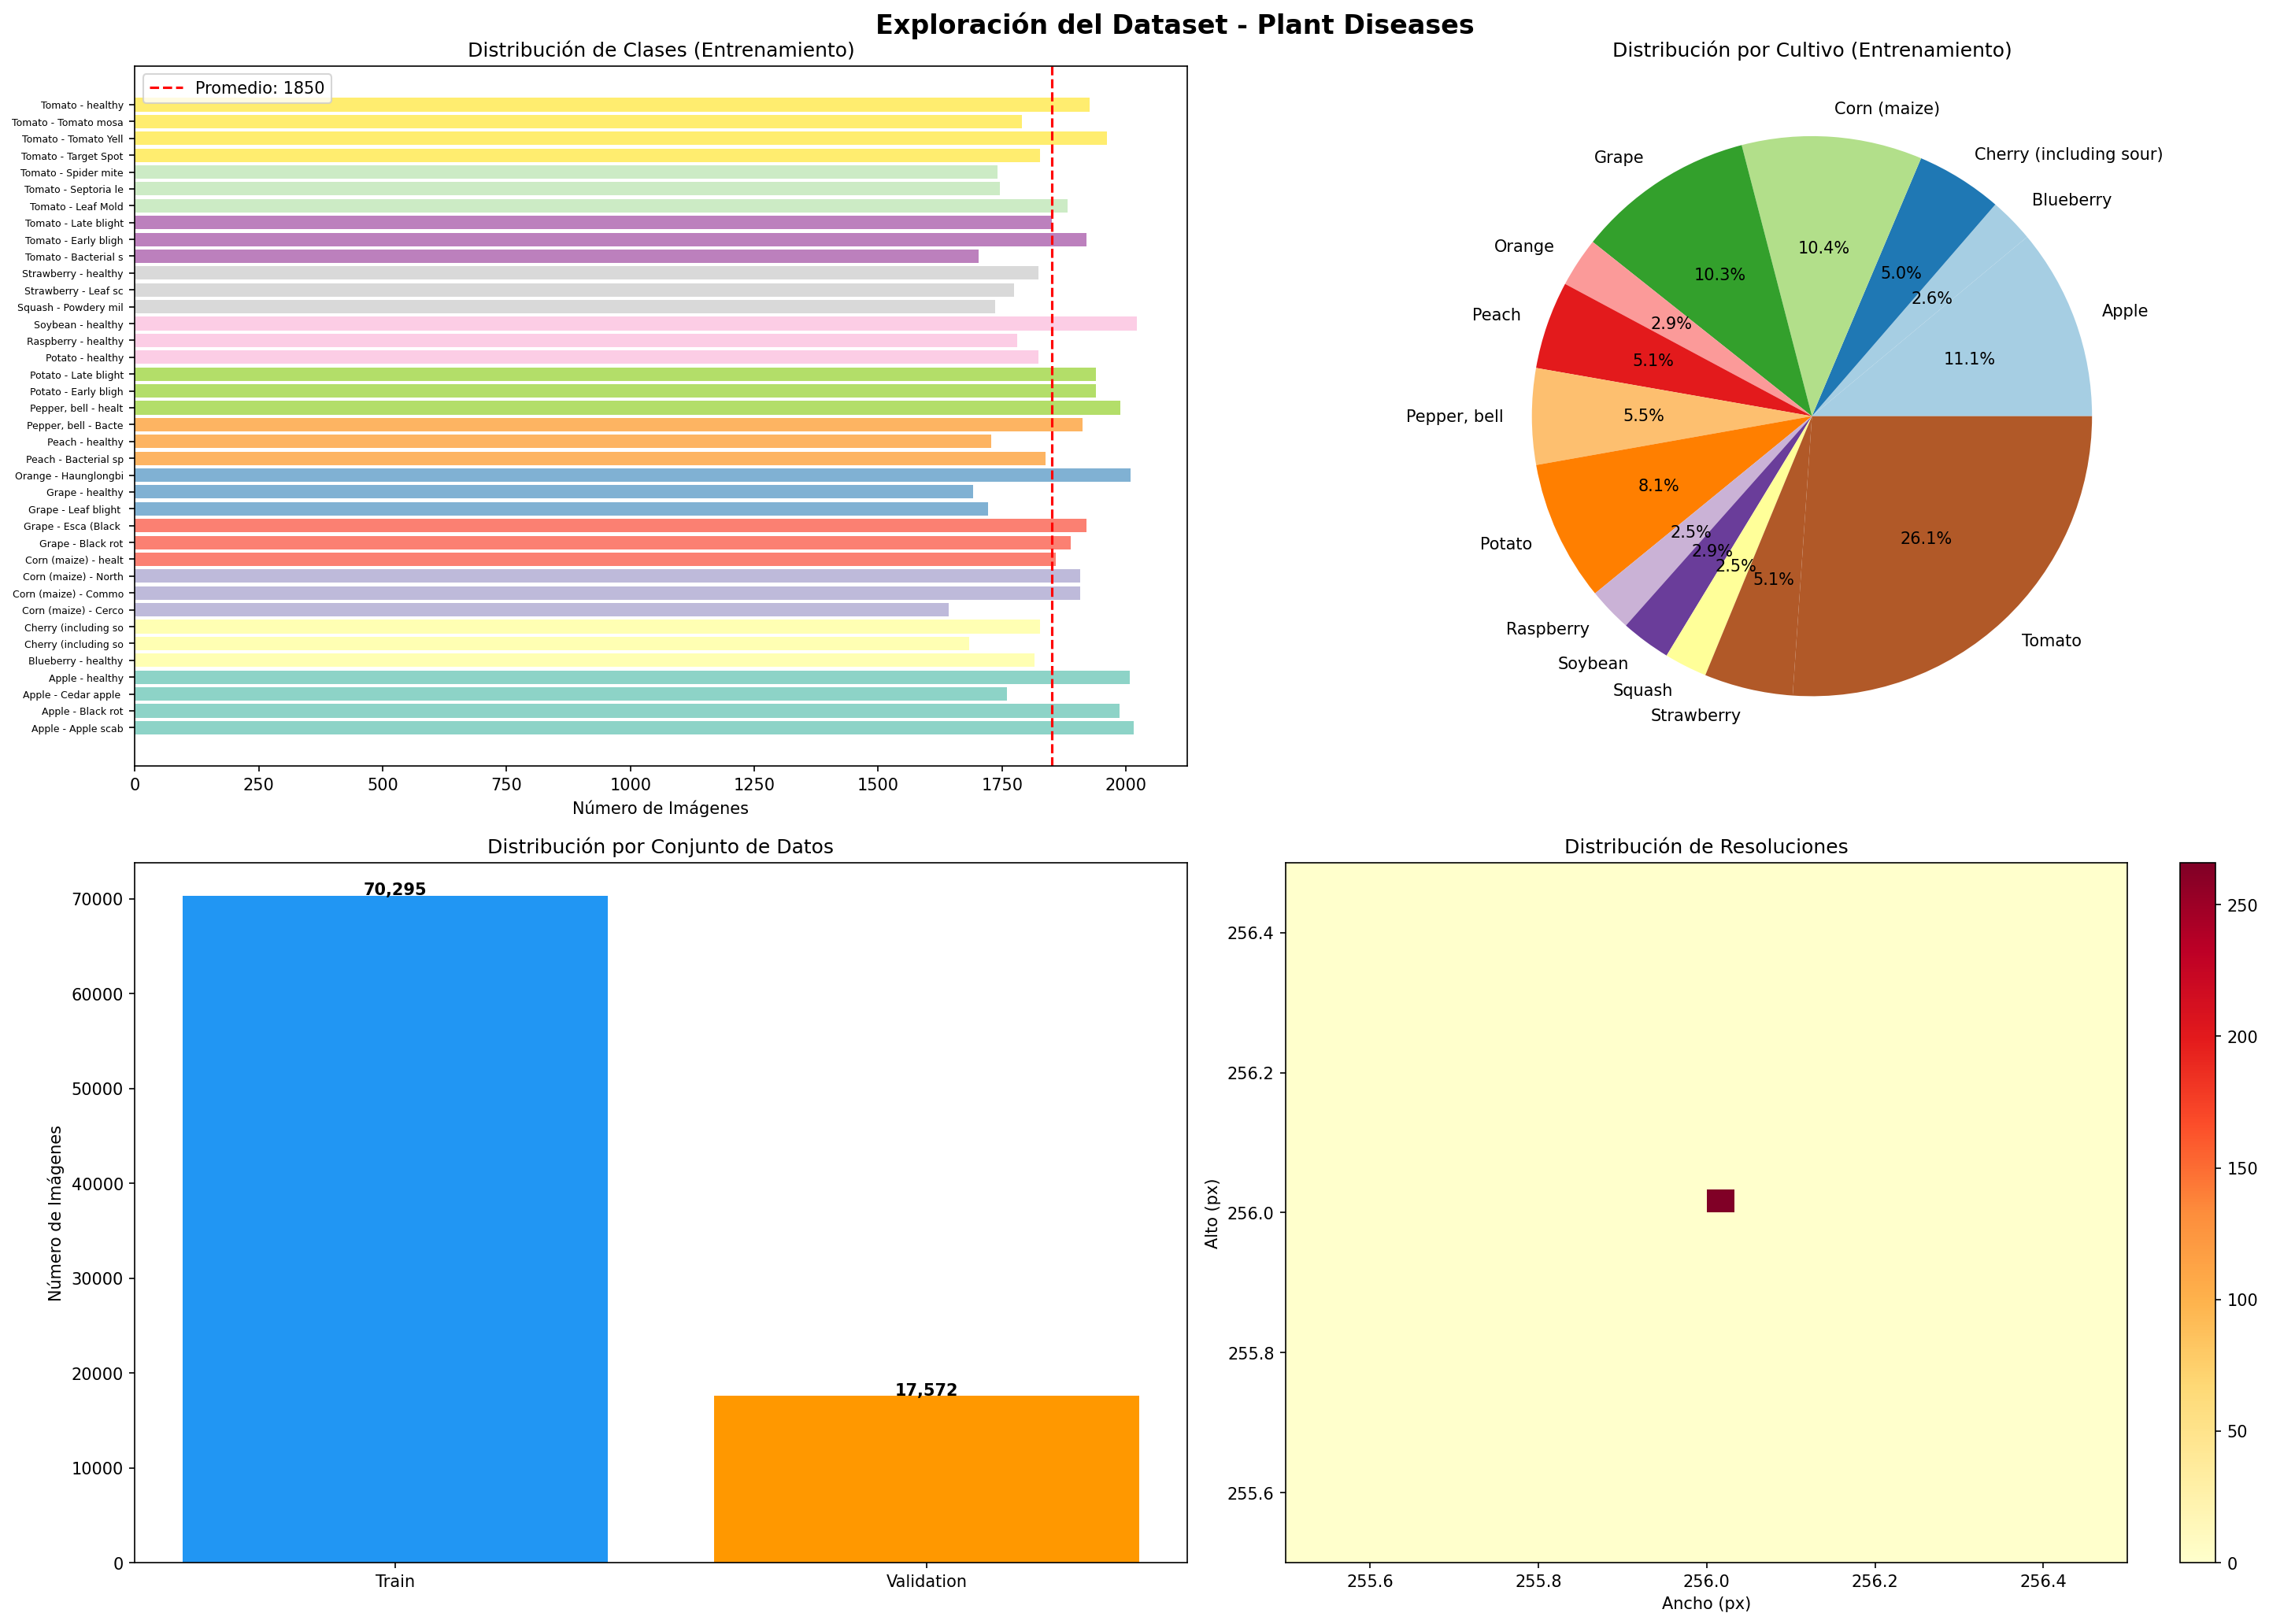
\includegraphics[width=0.62\textwidth]{images/eda_analysis.png}
  \vspace{0.2cm}
  \footnotesize
  \begin{itemize}
    \item Dataset razonablemente balanceado: entre 1{,}650 y 2{,}020 imágenes por clase (promedio 1{,}850).
    \item \textbf{Tomate} concentra el 26\% de las imágenes (10 subtipos de enfermedad); el resto se reparte entre 13 cultivos más.
    \item División 80/20: 70{,}295 imágenes de entrenamiento y 17{,}572 de validación.
    \item Prácticamente todas las imágenes vienen ya normalizadas a 256$\times$256 px.
  \end{itemize}
\end{frame}

\begin{frame}{Fase 2 — Preprocesamiento y Data Augmentation}
  \begin{itemize}
    \item Se generó \texttt{class\_mapping.json}: traduce cada clase técnica (ej. \texttt{Tomato\_\_\_Early\_blight}) a \textit{cultivo} + \textit{enfermedad} en español — pieza clave que usa la API para responder.
    \item Se configuró \textbf{Data Augmentation} (rotación, zoom, brillo, flip horizontal) para mejorar la generalización del modelo.
  \end{itemize}
\end{frame}

\begin{frame}{Fase 2 — Distribución tras el preprocesamiento}
  \centering
  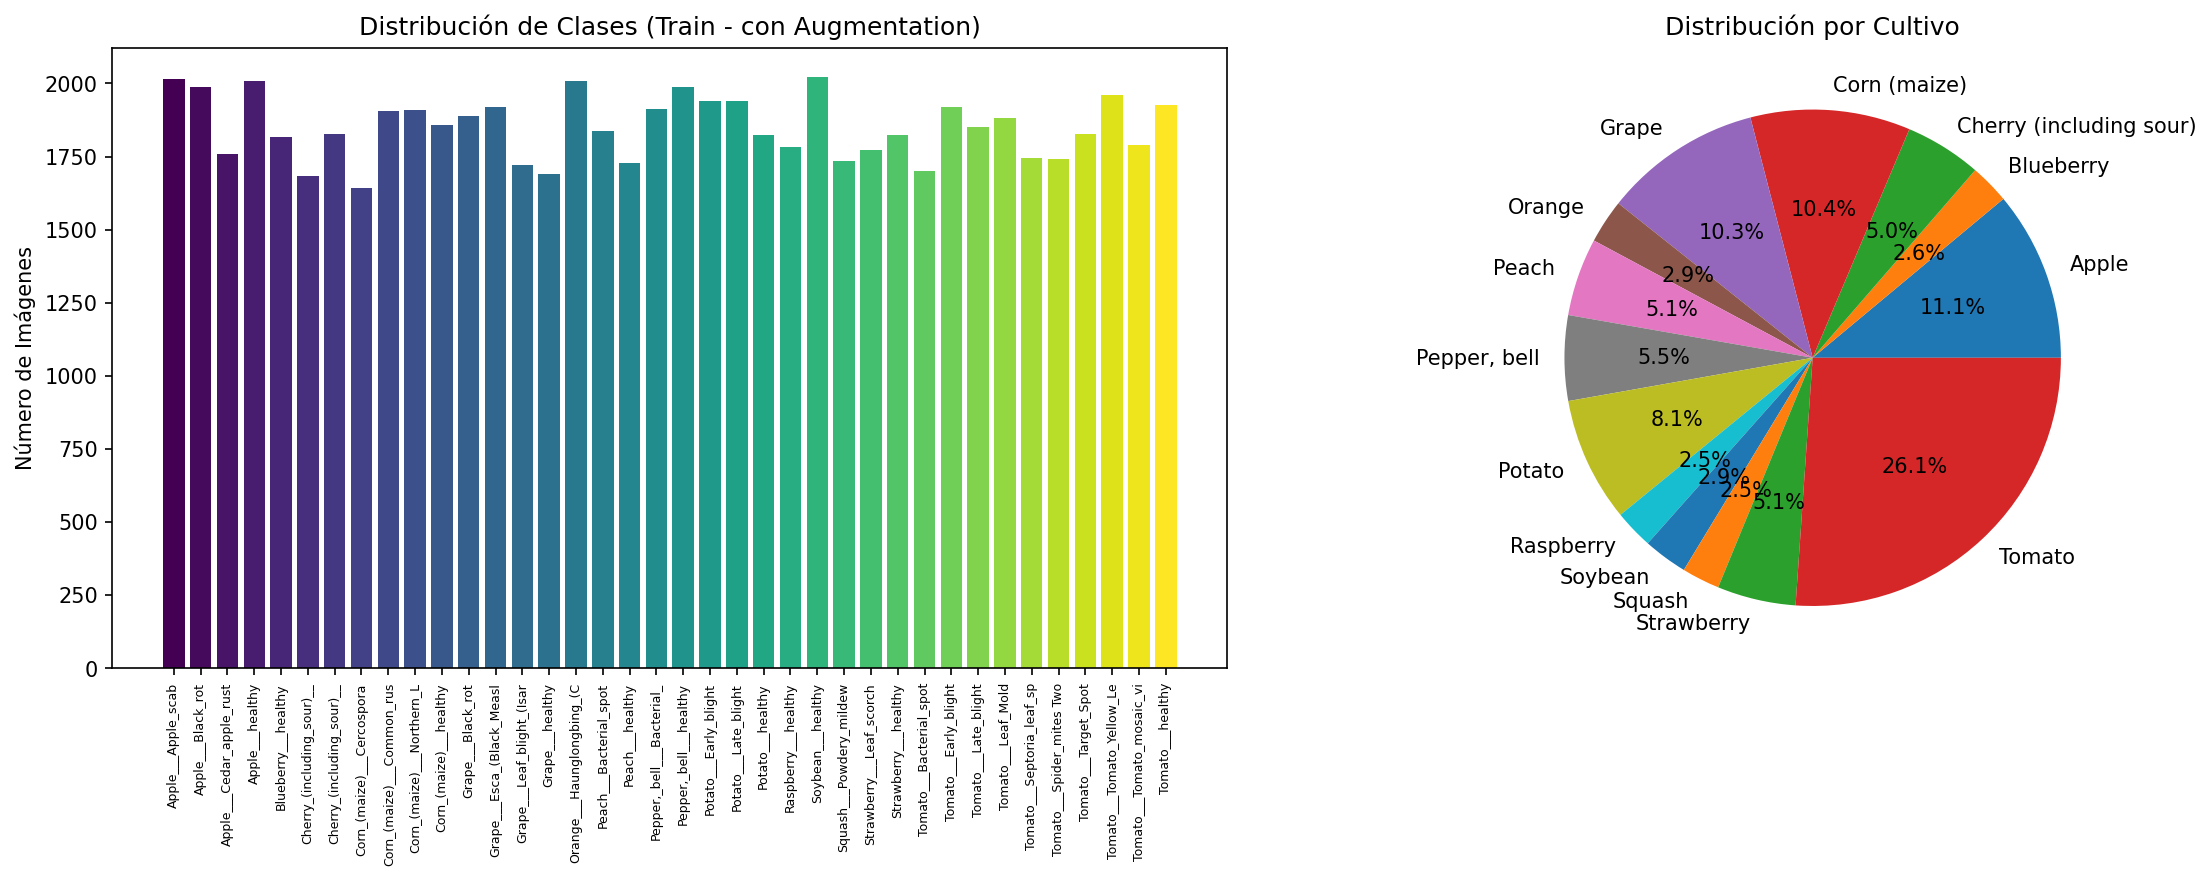
\includegraphics[width=0.58\textwidth]{images/class_distribution_preprocessed.png}
  \vspace{0.2cm}
  \footnotesize
  \begin{itemize}
    \item Tras el Data Augmentation la distribución por clase queda aún más pareja (todas entre 1{,}650 y 2{,}020 imágenes).
    \item Las proporciones por cultivo se mantienen igual que en el EDA; el objetivo no era cambiar el balance entre cultivos, sino asegurar suficientes ejemplos por cada clase individual.
  \end{itemize}
\end{frame}

\begin{frame}{Fase 2 — Ejemplo de Data Augmentation}
  \centering
  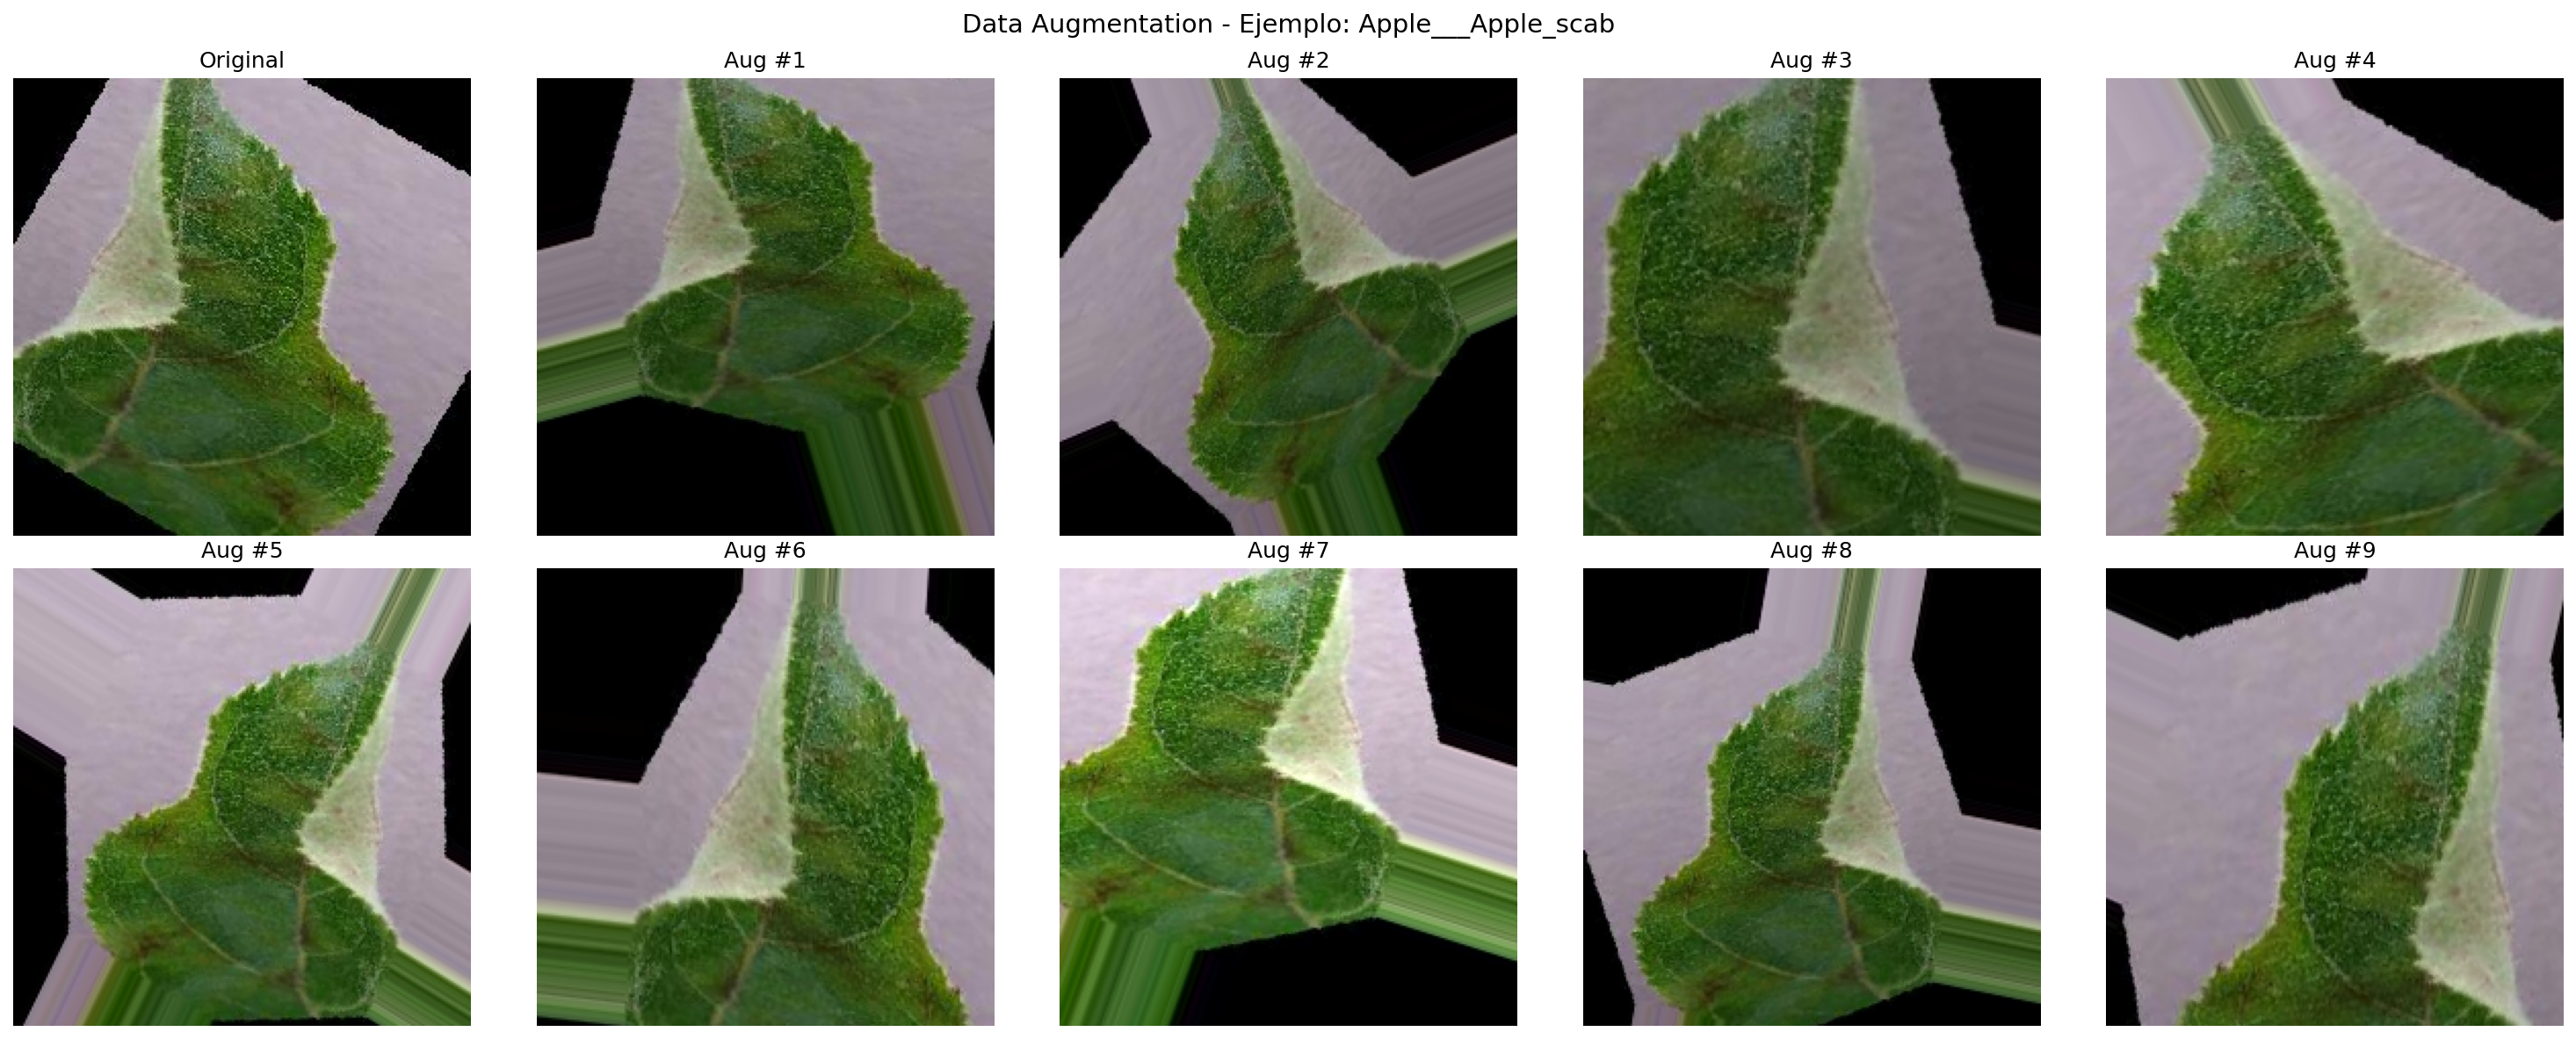
\includegraphics[width=0.68\textwidth]{images/data_augmentation_example.png}
  \vspace{0.2cm}
  \footnotesize
  \begin{itemize}
    \item Misma hoja transformada 9 veces: rotaciones, recortes/zoom y cambios de color/brillo.
    \item Las variaciones son visuales, no alteran el patrón de la enfermedad — el objetivo es que el modelo no memorice el ángulo o la iluminación exacta de cada foto, sino la forma y textura de la lesión.
  \end{itemize}
\end{frame}

\begin{frame}{Fase 3 — CNN propia: resultado}
  \begin{block}{Arquitectura}
    4 bloques convolucionales (32 $\to$ 64 $\to$ 128 $\to$ 256 filtros) con BatchNorm y Dropout, sin usar ningún modelo preentrenado.
  \end{block}
  \begin{itemize}
    \item Entrenada en Kaggle mediante \textbf{``Save Version''} (ejecución en segundo plano, no depende de mantener el navegador abierto).
    \item \textbf{Resultado: $\approx$ 99.7\% de accuracy en validación.}
    \item Checkpoint del mejor modelo (\texttt{cnn\_custom\_best.keras}) descargado y ya integrado al proyecto local.
    \item Detalle menor: la sesión de Kaggle se cortó justo después de guardar el mejor checkpoint, por lo que no se generaron el modelo ``final'' ni el JSON de métricas — no es bloqueante, la API solo necesita el ``best''.
  \end{itemize}
\end{frame}

\begin{frame}{Fase 3 — Resultado CNN Propia}
  \centering
  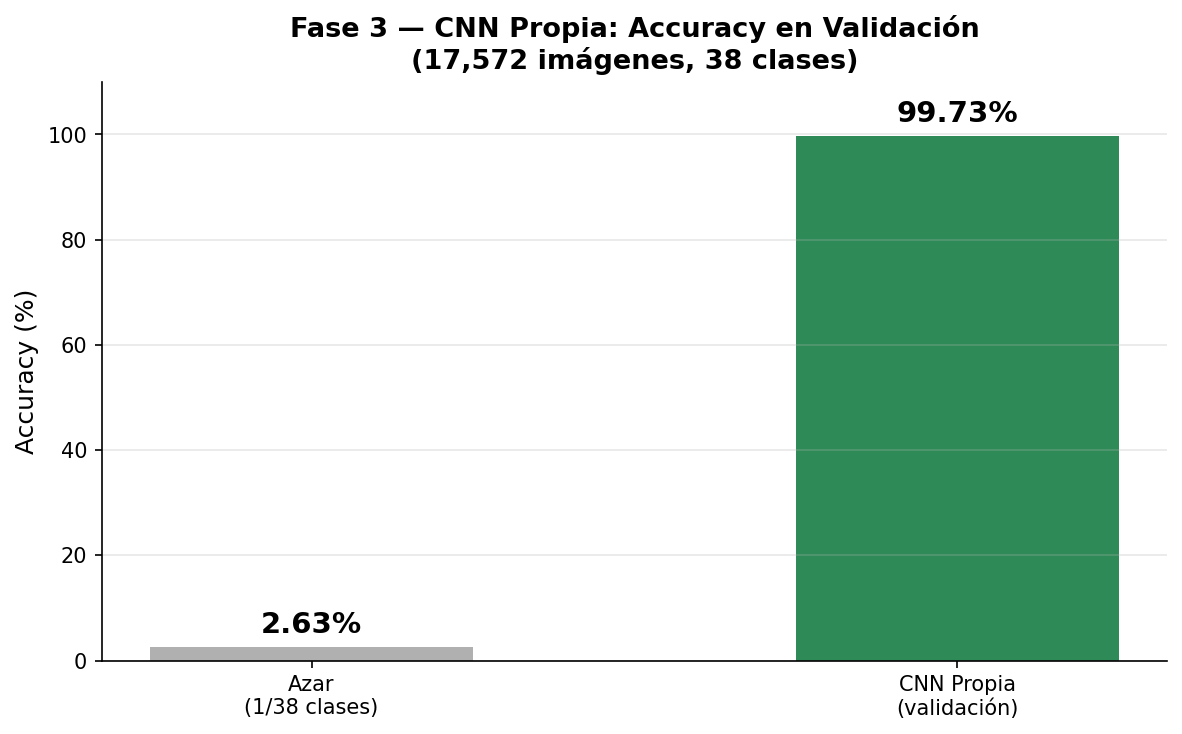
\includegraphics[width=0.52\textwidth]{images/cnn_custom_result.png}
  \vspace{0.2cm}
  \footnotesize
  \begin{itemize}
    \item 99.73\% de accuracy en validación, muy por encima del azar (2.63\%, equivalente a acertar 1 de 38 clases).
    \item Confirma que el modelo aprendió patrones reales de las imágenes y no está adivinando.
  \end{itemize}
  \vspace{0.15cm}
  \footnotesize Nota: no se generaron las curvas de entrenamiento por época (\texttt{cnn\_custom\_training.png}) porque la sesión de Kaggle se cortó antes de esa etapa final del script; el valor mostrado es el accuracy real del checkpoint guardado.
\end{frame}

\begin{frame}{Fase 4 — Intento 1: entrenamiento local}
  \begin{itemize}
    \item Se lanzó el entrenamiento localmente usando la GPU del equipo (RTX 3050 laptop) con el dataset ya descargado.
    \item El proceso \textbf{se interrumpió antes de terminar} (aprox. 6 horas después de iniciado, sin actividad posterior) — muy probablemente por suspensión del equipo o cierre de la sesión.
    \item Se recuperó únicamente un checkpoint intermedio, guardado automáticamente durante el entrenamiento.
  \end{itemize}
\end{frame}

\begin{frame}{Fase 4 — Verificación del checkpoint recuperado}
  \begin{itemize}
    \item Se cargó el checkpoint y se evaluó contra las 17{,}572 imágenes de validación.
  \end{itemize}
  \begin{alertblock}{Resultado de la verificación}
    \textbf{Val Accuracy: 23.9\%} — \quad \textbf{Val Loss: 4.72}
  \end{alertblock}
  \begin{itemize}
    \item Muy por debajo de lo esperado para ResNet50 con transfer learning (normalmente 85–95\%+ en este dataset).
    \item Confirma que el entrenamiento se cortó en una etapa muy temprana. \textbf{El checkpoint no es utilizable.}
  \end{itemize}
\end{frame}

\begin{frame}{Fase 4 — Decisión y siguiente intento}
  \begin{itemize}
    \item Dado que el enfoque ``Save Version'' de Kaggle funcionó de forma confiable para la CNN propia (corre en segundo plano, sin depender del navegador ni de la laptop encendida), se decidió repetir el mismo enfoque para ResNet50.
    \item Script \texttt{kaggle\_notebook/04\_transfer\_learning.py} ya ajustado y listo para lanzar.
  \end{itemize}
  \begin{block}{Estimación de tiempo}
    Completar las 30 épocas configuradas para ResNet50 (23M+ parámetros, últimas 30 capas descongeladas, $\sim$70k imágenes de entrenamiento) tomaría aproximadamente \textbf{8 a 10 horas} de cómputo continuo.
  \end{block}
\end{frame}

\begin{frame}{Fase 4 — Resultado final: entrenamiento completado}
  \begin{block}{Segundo intento en Kaggle}
    Esta vez el entrenamiento corrió sin interrupciones: \textbf{30 épocas completas en $\sim$8.7 horas}, tal como se había estimado.
  \end{block}
  \begin{itemize}
    \item \textbf{Accuracy de validación: 76.9\%}
    \item Modelo final descargado e integrado al proyecto (\texttt{resnet50\_best.keras}).
  \end{itemize}
\end{frame}

\begin{frame}{Fase 4 — Curvas de entrenamiento}
  \centering
  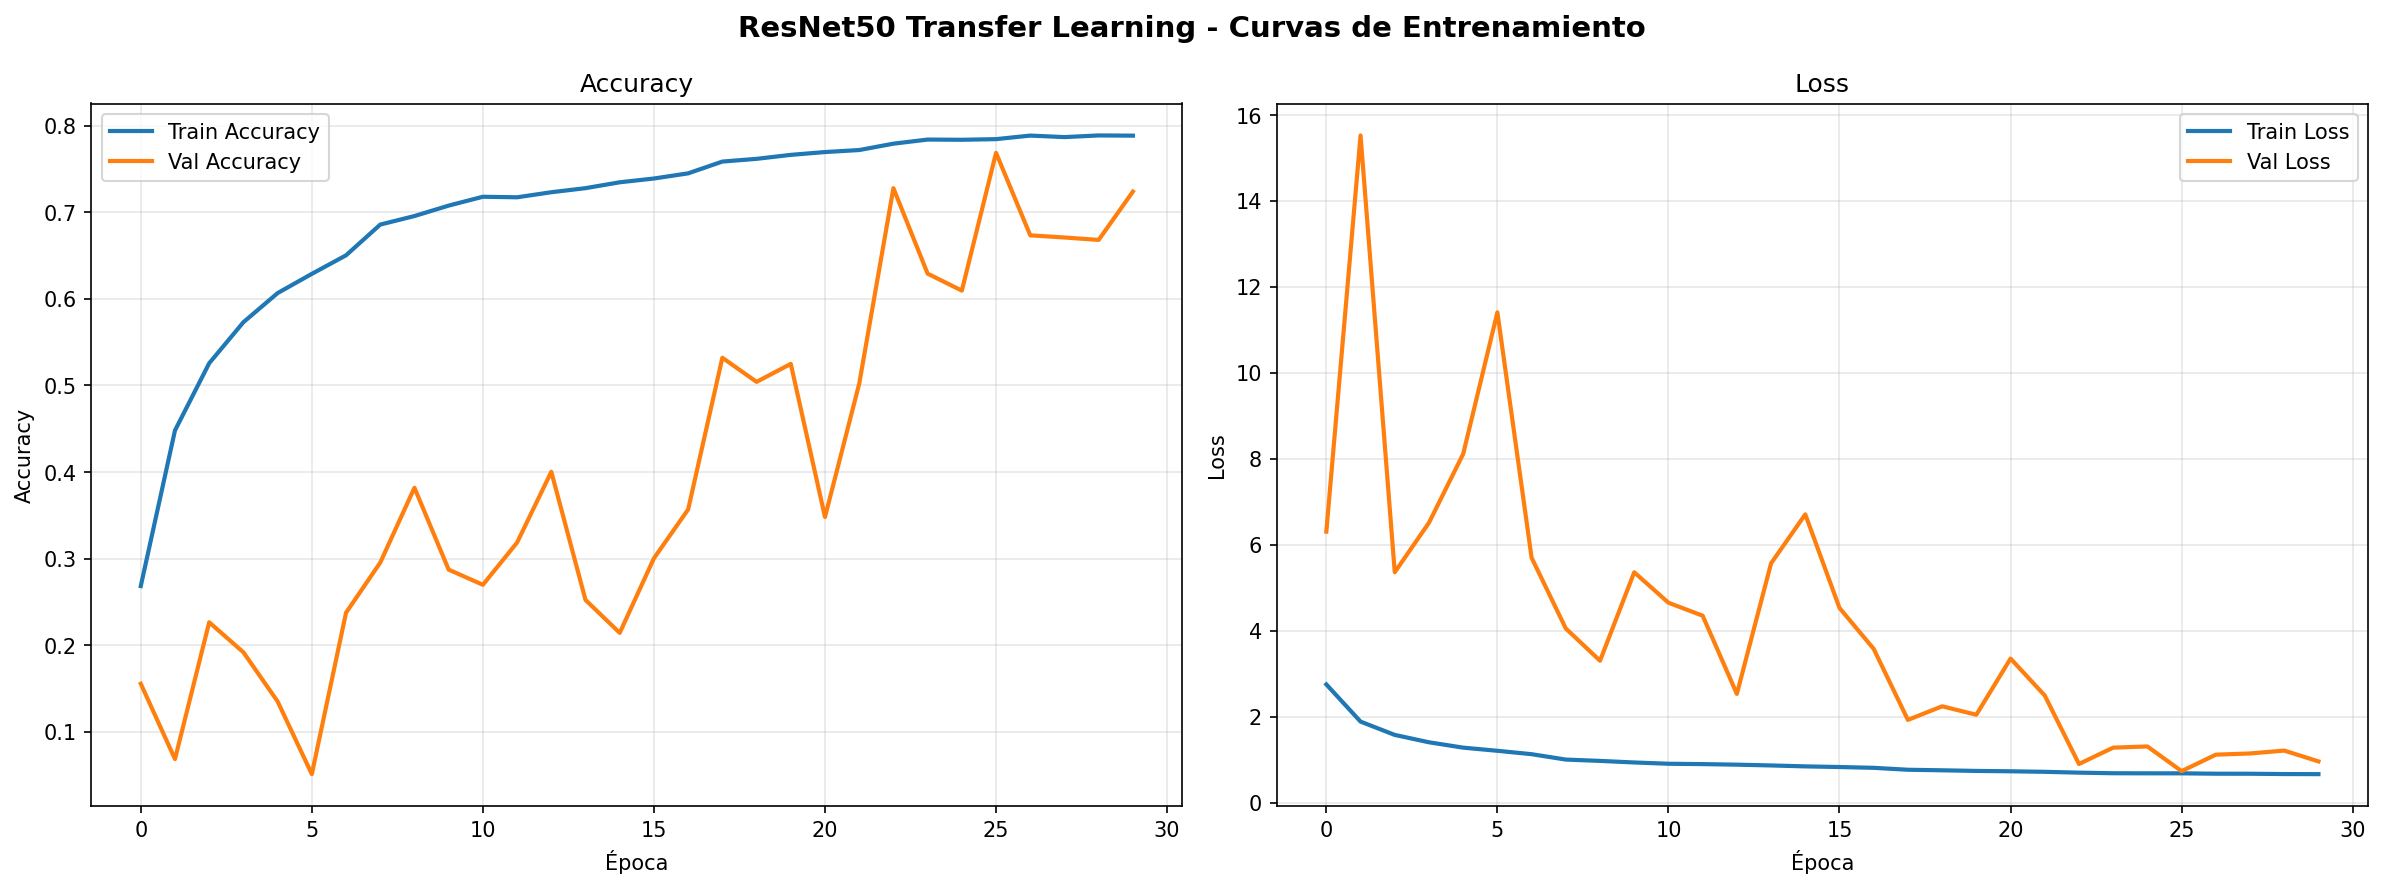
\includegraphics[width=0.62\textwidth]{images/resnet50_training.png}
  \vspace{0.2cm}
  \footnotesize
  \begin{itemize}
    \item El accuracy de entrenamiento sube de forma estable hasta $\sim$78\%; el de validación es mucho más ruidoso (sube y baja bruscamente de época a época), aunque la tendencia general también es a mejorar.
    \item El mejor checkpoint se guardó en la época 26 (76.9\% val accuracy) — el ruido en validación es normal al descongelar capas de un modelo grande; por eso se usa \texttt{ModelCheckpoint} con el mejor punto, no la última época.
  \end{itemize}
\end{frame}

\begin{frame}{Fase 5 — CNN propia vs. ResNet50}
  \centering
  \begin{tabular}{lcc}
    \toprule
    \textbf{Métrica} & \textbf{CNN propia} & \textbf{ResNet50} \\
    \midrule
    Accuracy & 99.7\% & 76.9\% \\
    Precisión & 99.7\% & 80.7\% \\
    Recall & 99.7\% & 76.9\% \\
    F1-score & 99.7\% & 75.8\% \\
    \bottomrule
  \end{tabular}
  \vspace{0.4cm}
  \begin{itemize}
    \item La CNN propia superó claramente a ResNet50 en este dataset.
    \item Se generaron matrices de confusión, curvas ROC y métricas por clase para ambos modelos (\texttt{reports/}).
  \end{itemize}
\end{frame}

\begin{frame}{Fase 5 — Comparación final de métricas}
  \centering
  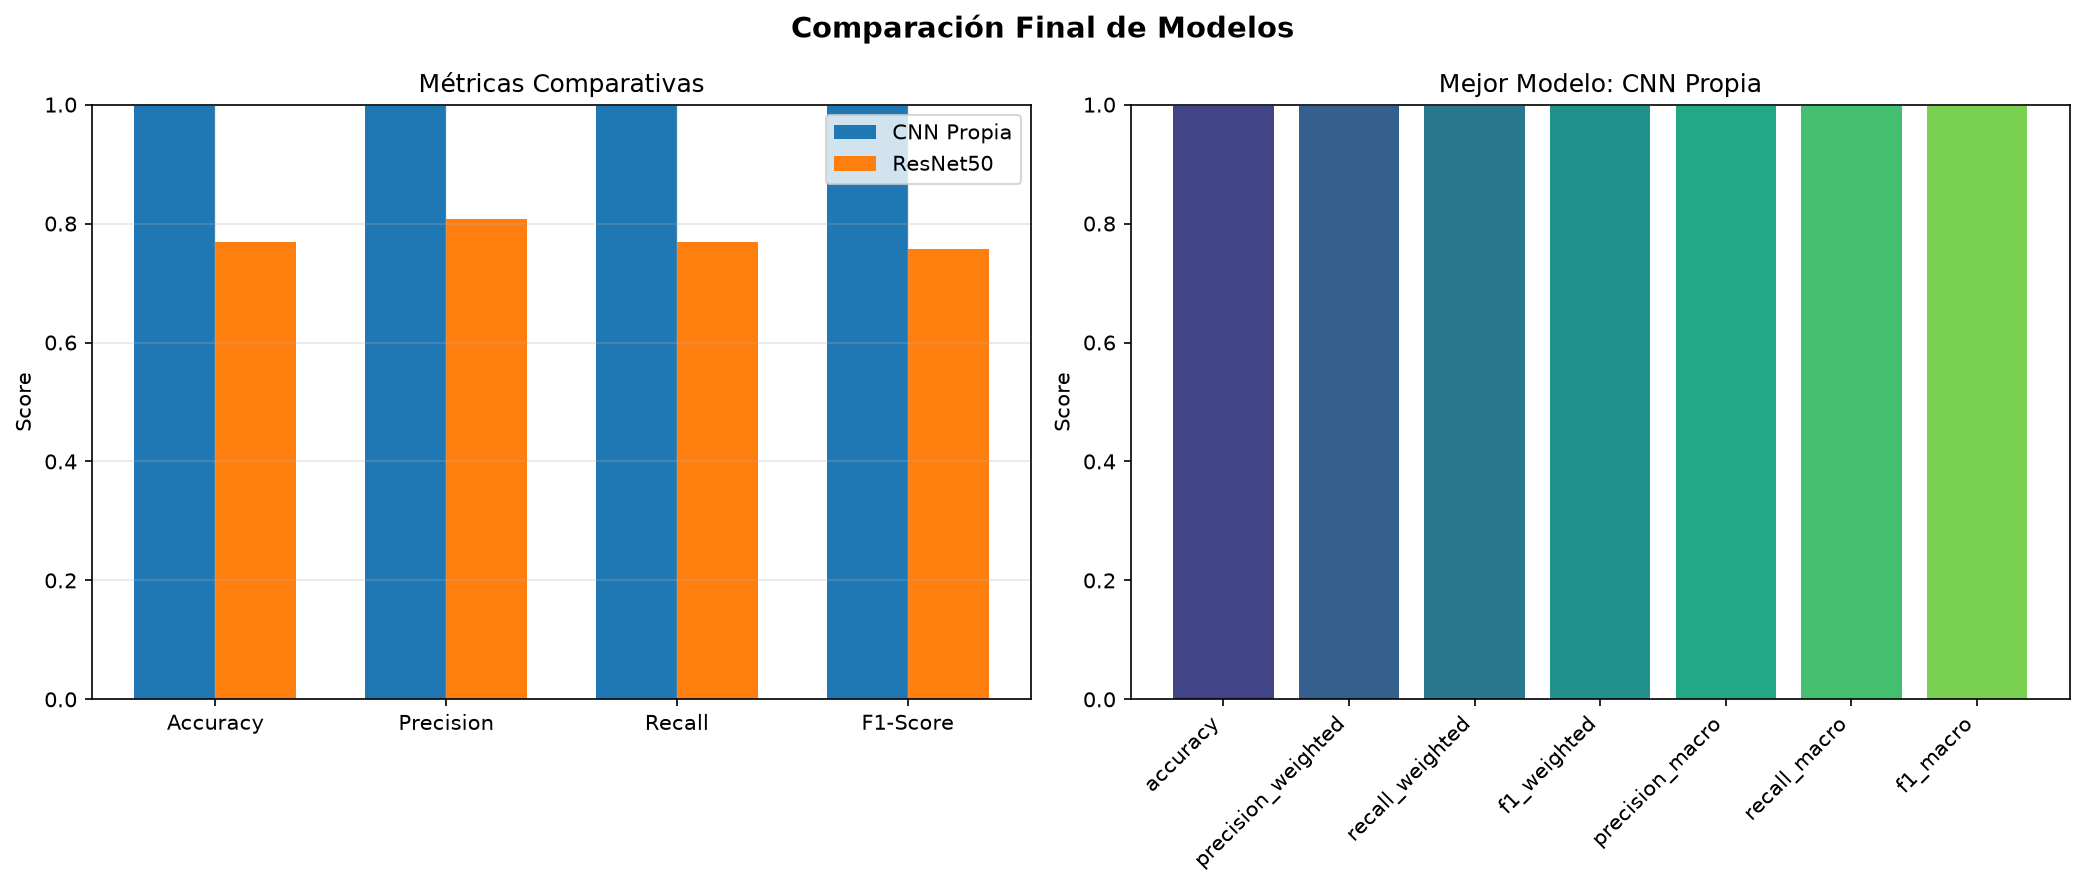
\includegraphics[width=0.72\textwidth]{images/final_comparison.png}
  \vspace{0.2cm}
  \footnotesize
  \begin{itemize}
    \item Izquierda: la CNN propia gana en las 4 métricas frente a ResNet50, no solo en accuracy.
    \item Derecha: el resultado de la CNN propia es igual de alto en promedio ponderado (\textit{weighted}, pondera por cantidad de imágenes por clase) que en promedio simple (\textit{macro}, todas las clases pesan igual) — es decir, no le va bien solo en las clases con más imágenes, sino en todas por igual.
  \end{itemize}
\end{frame}

\begin{frame}{Fase 5 — Matrices de confusión}
  \centering
  \begin{columns}[T]
    \begin{column}{0.48\textwidth}
      \centering
      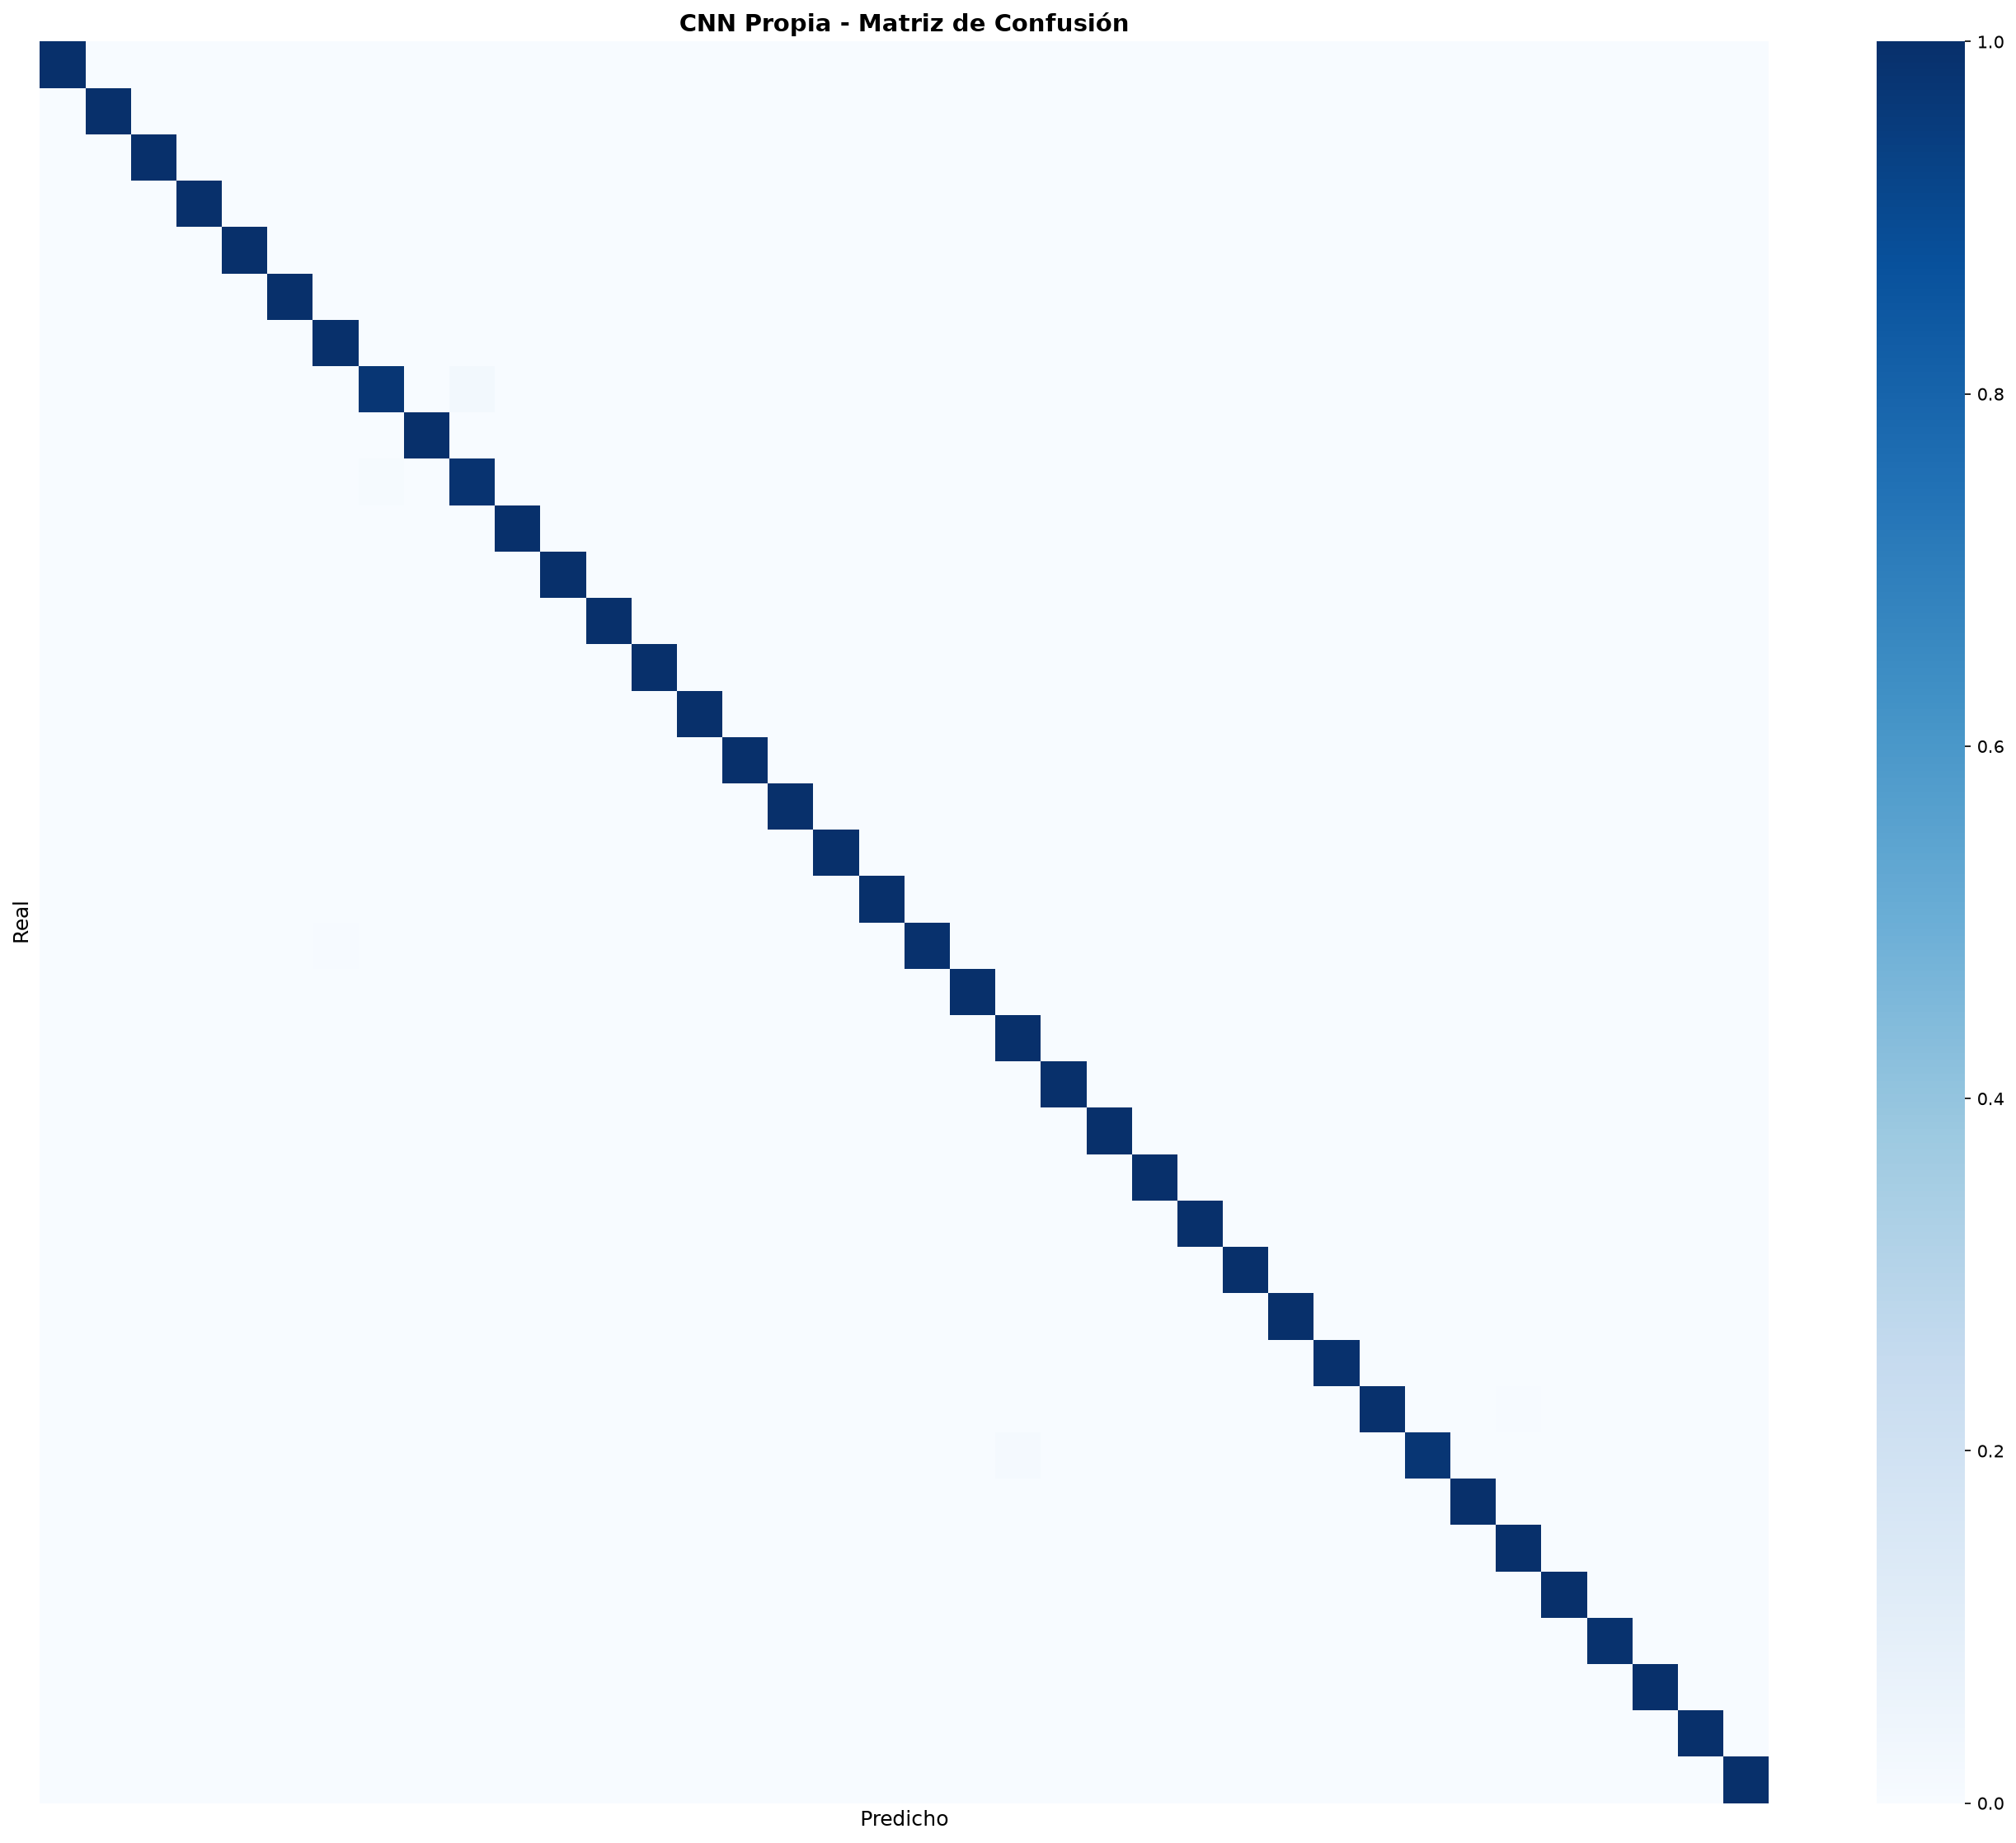
\includegraphics[width=\textwidth]{images/cnn_propia_confusion_matrix.png}\\
      \footnotesize CNN Propia
    \end{column}
    \begin{column}{0.48\textwidth}
      \centering
      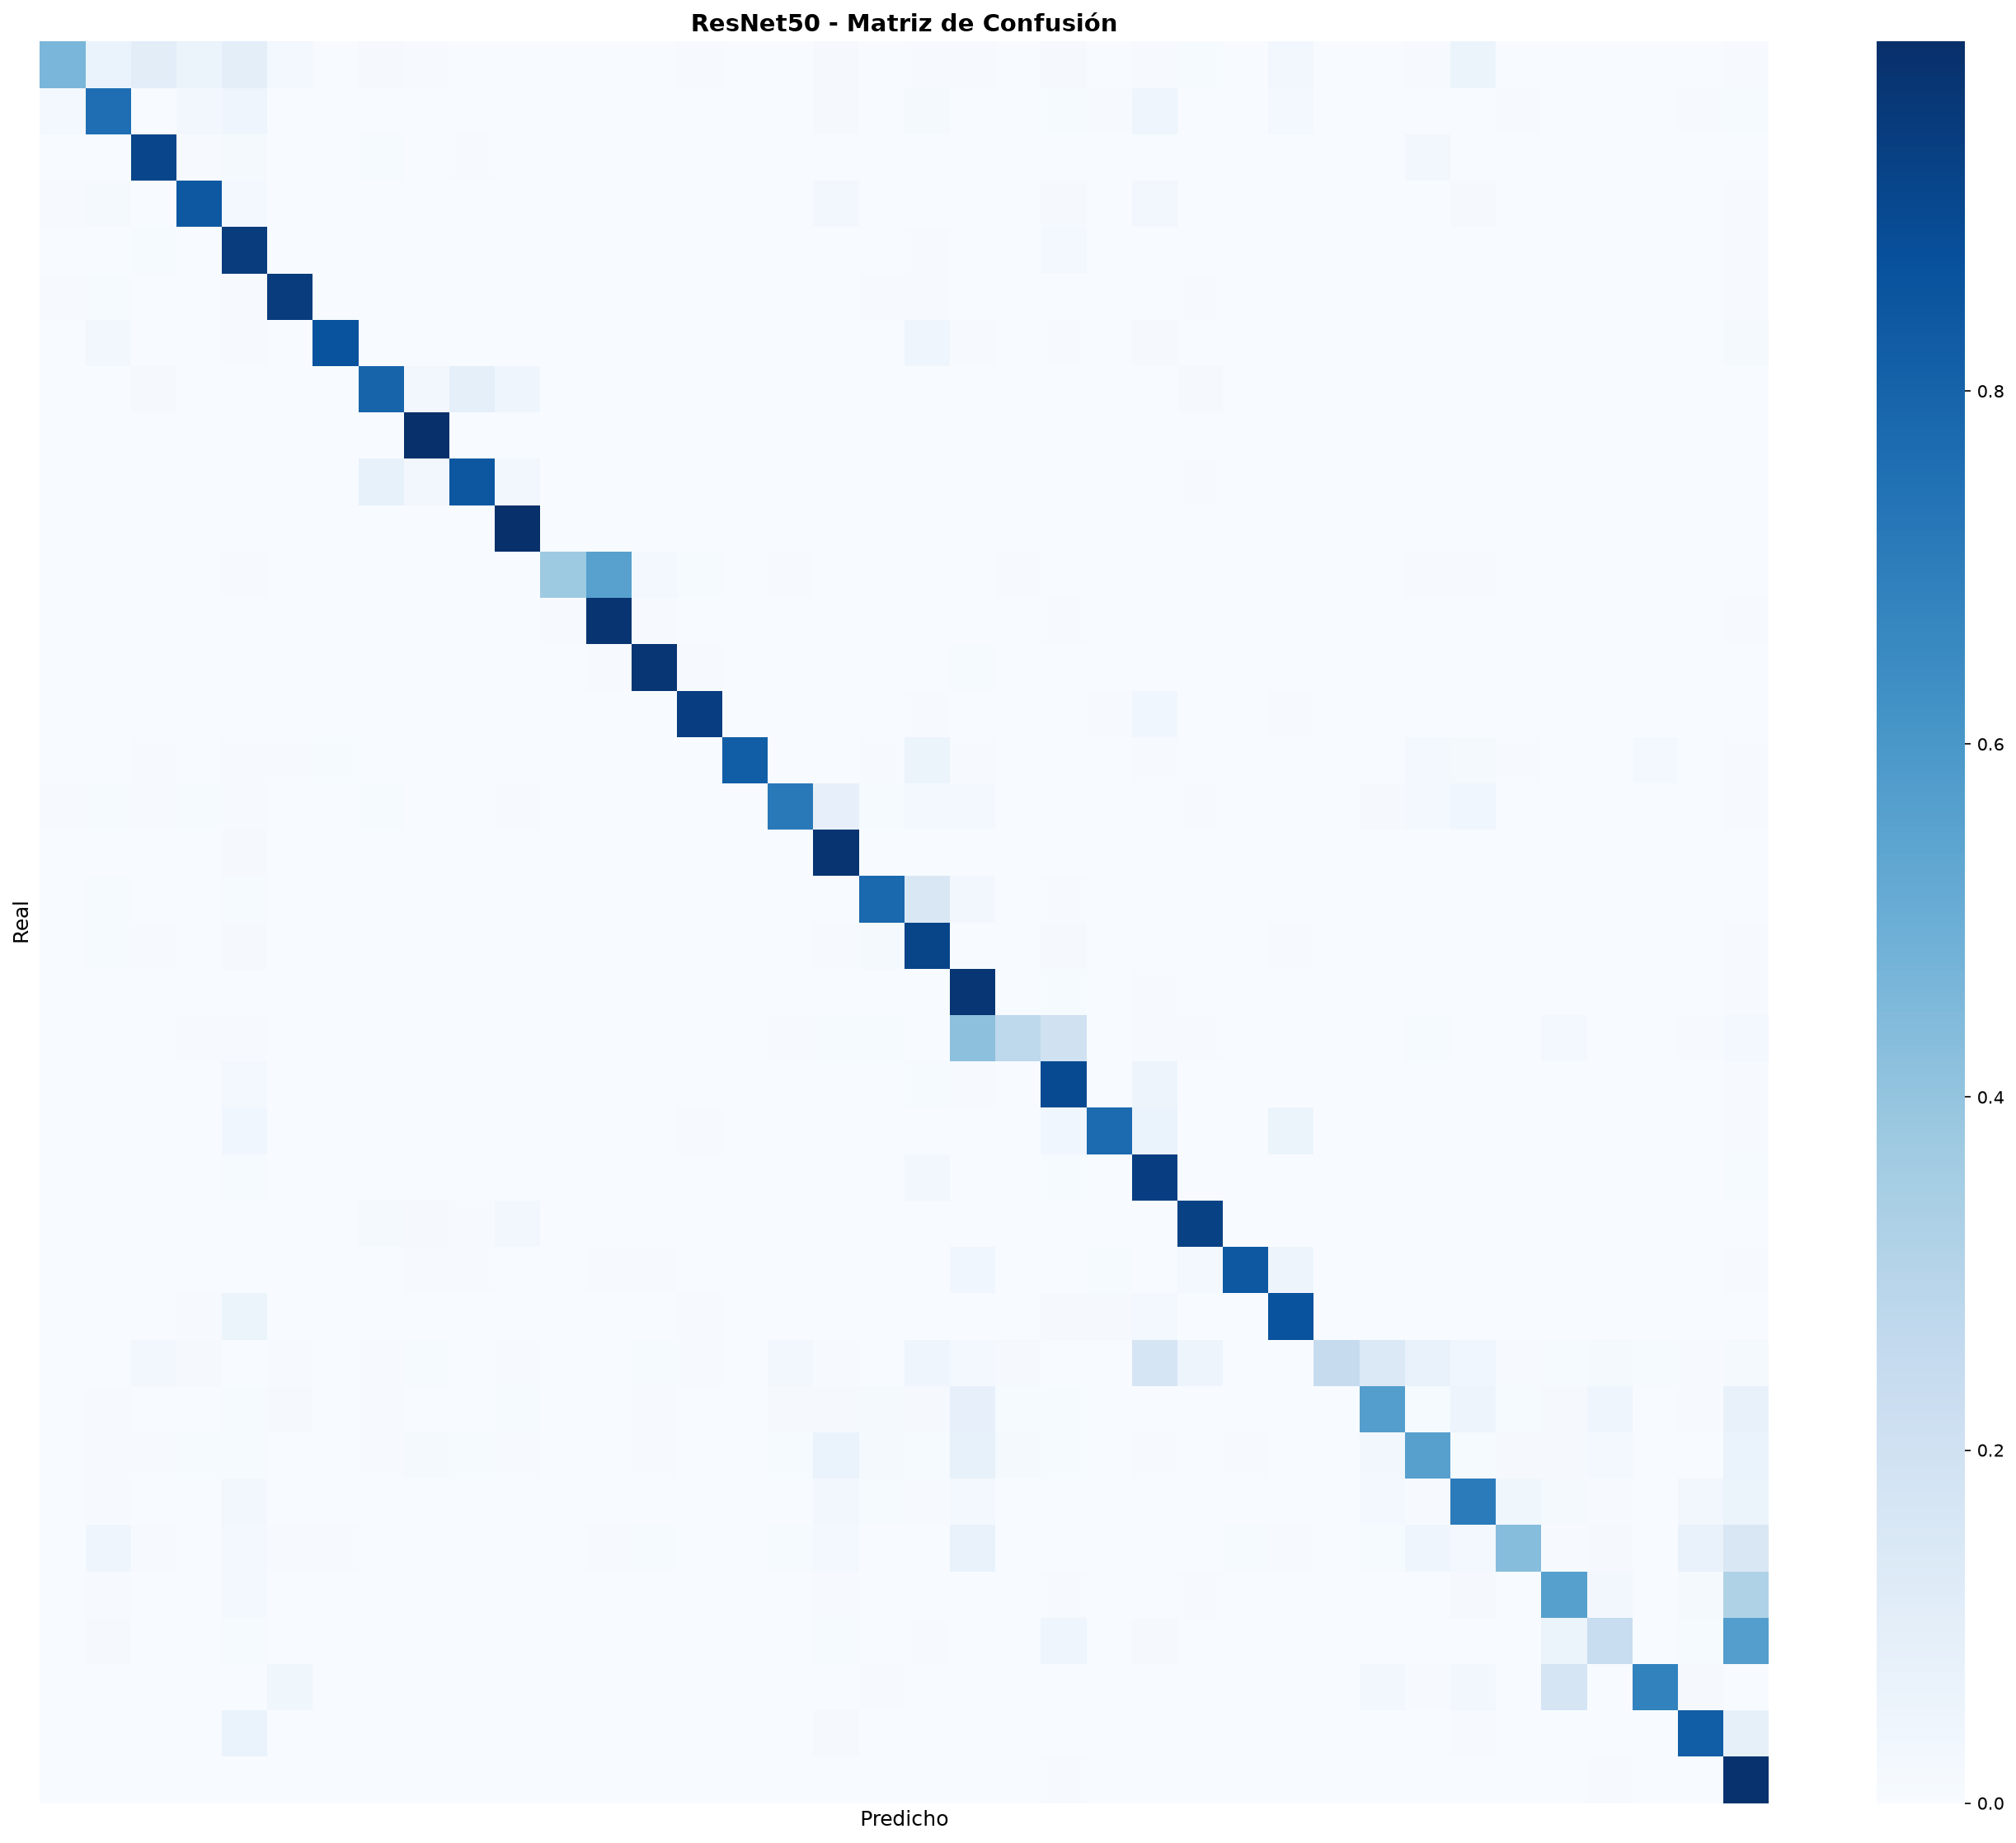
\includegraphics[width=\textwidth]{images/resnet50_confusion_matrix.png}\\
      \footnotesize ResNet50
    \end{column}
  \end{columns}
  \vspace{0.3cm}
  \footnotesize
  \begin{itemize}
    \item La diagonal de la CNN propia es prácticamente sólida (casi sin errores visibles).
    \item ResNet50 también acierta en la mayoría de los casos, pero muestra más confusión con clases vecinas — típicamente distintas enfermedades de un mismo cultivo, que se parecen más entre sí visualmente.
  \end{itemize}
\end{frame}

\begin{frame}{Fase 6 — Despliegue con Docker}
  \begin{itemize}
    \item Imagen basada en \texttt{python:3.11-slim}, con \texttt{gunicorn} sirviendo la API (2 workers).
    \item \texttt{HEALTHCHECK} integrado (\texttt{curl /health} cada 30s) para que Docker detecte si el servicio deja de responder.
    \item \texttt{.dockerignore} excluye dataset, entorno virtual y material que no necesita el contenedor.
  \end{itemize}
  \begin{alertblock}{Reto real encontrado y corregido}
    El contenedor fallaba al cargar el modelo por una incompatibilidad de versión de Keras: la imagen base solo permitía instalar una versión más antigua que la usada para guardar los modelos. Se corrigió actualizando la imagen base y fijando la versión exacta de Keras en \texttt{requirements.txt}.
  \end{alertblock}
\end{frame}

\begin{frame}{Fase 7 — Frontend: resultado}
  \centering
  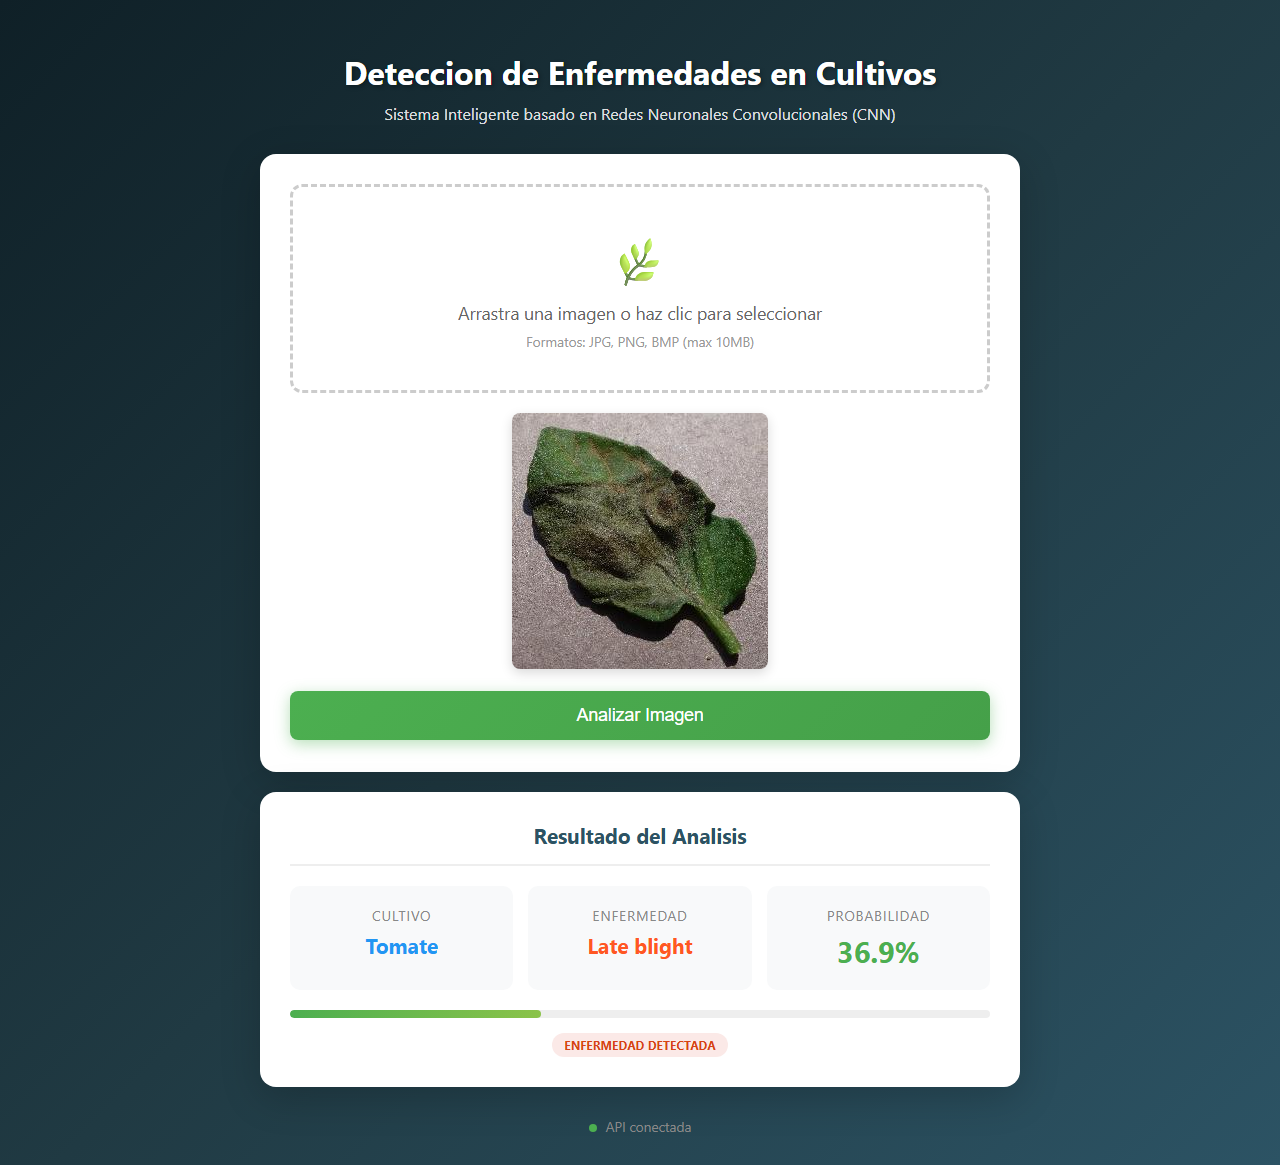
\includegraphics[width=0.42\textwidth]{images/frontend_resultado.png}
  \vspace{0.15cm}
  \footnotesize
  \begin{itemize}
    \item Selección de imagen por arrastrar-y-soltar o clic, con vista previa antes de analizar.
    \item Indicador de conexión con la API en tiempo real (\textit{``API conectada''}, vía \texttt{/health}).
    \item Resultado mostrado con cultivo, enfermedad, probabilidad (barra animada) y etiqueta de estado.
    \item Probado de extremo a extremo: subir imagen $\to$ analizar $\to$ ver resultado, servido desde el mismo contenedor Docker.
  \end{itemize}
\end{frame}

% ===========================================================
\section{Limitaciones y dificultades}

\begin{frame}{Limitaciones encontradas}
  \begin{itemize}
    \item \textbf{Tamaño del dataset ($\sim$3\,GB)}: la descarga local fue extremadamente lenta, forzando el cambio de estrategia hacia Kaggle.
    \item \textbf{Cuotas de Kaggle}: sesiones gratuitas de GPU limitadas ($\sim$9–12 h por sesión, $\sim$30 h/semana), lo que restringe cuántos reintentos se pueden hacer.
    \item \textbf{Interrupciones de entrenamiento}: tanto local (suspensión del equipo) como en Kaggle (corte de sesión antes de guardar artefactos finales de la CNN).
    \item \textbf{Hardware local limitado}: GPU de laptop (RTX 3050) suficiente para validar checkpoints, pero no ideal para entrenar ResNet50 completo en tiempos cortos.
    \item \textbf{Tiempo de cómputo de ResNet50}: al ser un modelo mucho más pesado que la CNN propia, su entrenamiento completo tomó cerca de 9 horas.
  \end{itemize}
\end{frame}

% ===========================================================
\section{Estado final del proyecto}

\begin{frame}{Resumen del estado final}
  \centering
  \begin{tabular}{p{5.2cm}p{3.5cm}}
    \toprule
    \textbf{Fase} & \textbf{Estado} \\
    \midrule
    Fase 1 — Exploración (EDA) & \textcolor{okgreen}{\textbf{Completada}} \\
    Fase 2 — Preprocesamiento y Augmentation & \textcolor{okgreen}{\textbf{Completada}} \\
    Fase 3 — CNN propia & \textcolor{okgreen}{\textbf{Completada}} \\
    Fase 4 — Transfer Learning (ResNet50) & \textcolor{okgreen}{\textbf{Completada}} \\
    Fase 5 — Evaluación comparativa & \textcolor{okgreen}{\textbf{Completada}} \\
    Fase 6 — API + Docker & \textcolor{okgreen}{\textbf{Completada}} \\
    Fase 7 — Frontend & \textcolor{okgreen}{\textbf{Completada}} \\
    Subida a GitHub & \textcolor{okgreen}{\textbf{Completada}} \\
    \bottomrule
  \end{tabular}
\end{frame}

\begin{frame}{Estado final}
  \begin{enumerate}
    \item Ambos modelos entrenados y evaluados (accuracy, precision, recall, F1, matriz de confusión).
    \item API Flask probada localmente (\texttt{/predict}, \texttt{/health}) junto con el frontend web.
    \item Imagen Docker construida y probada de extremo a extremo (\texttt{/health}, \texttt{/predict}, frontend).
    \item Proyecto completo subido a GitHub.
  \end{enumerate}
\end{frame}

% ---------------------------------------------------------
\begin{frame}
  \centering
  \Large \textbf{¡Gracias!}\\[0.5cm]
  \normalsize Preguntas y comentarios
\end{frame}

\end{document}
